\section{Management \& Version Control Software}
For version control we are using git. To manage creating stories, logging time and creating burn down charts we are using JIRA which is deployed on one of our machines.
\section{Project management}
After a week of discussion on the game project idea, all main tasks were subdivided into Epics: \textit{level generation, GUI, game logic} and the \textit{character controller}. 

The epics are spread over the duration of the project and are broken down into a number of smaller stories as shown in figure~\ref{fig:backlog}. Tasks for each sprints will be chosen from the backlog based on their priority and requirements.

The project will be divided into 4 sprints. At the start of each week we will have a grooming and kick-off meeting. In the grooming meeting we will look through the backlog and see what stories we want to work on, assign story points and flesh out the descriptions or subtask them as required. In the kick-off we will assign tasks and give time estimates.

\begin{figure}[ht]
\centering
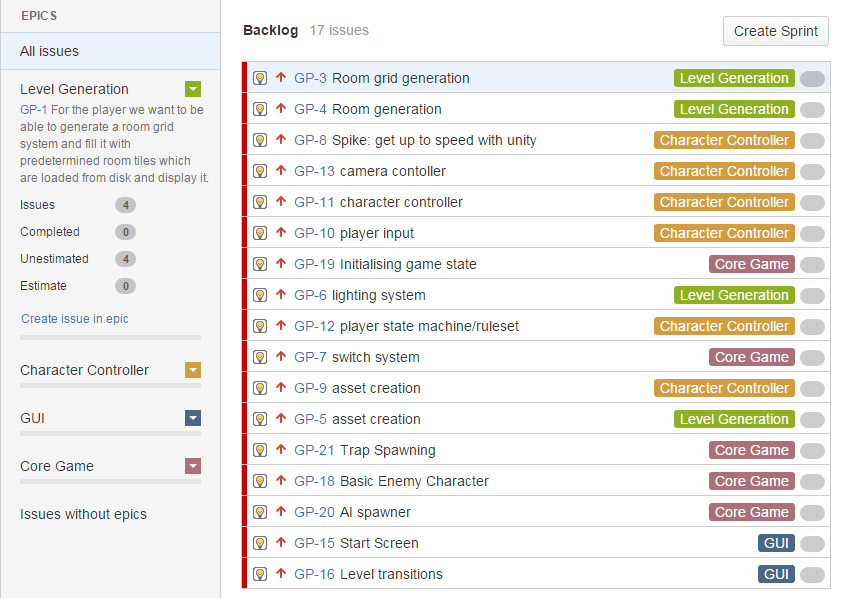
\includegraphics[scale = 0.8]{images/backlog.png}
\caption{Screenshot of Storyboard on Jira}
\label{fig:backlog}
\end{figure}
\section{Meeting Plan}
Sprint-Plan meetings would organized in the beginning of each sprint to discuss about the execution plan for the sprint tasks and Sprint-Demo meetings would be organised to discuss and demonstrate the executed sprint tasks.

The team will have stand-ups or kick-off/grooming meetings three times a week. Stand ups will aim to last for 10 minutes with any additional discussions happening in separate meetings outside this time.